\begin{center}

	
	
	\tikzset{every picture/.style={line width=0.75pt}} %set default line width to 0.75pt        
	
	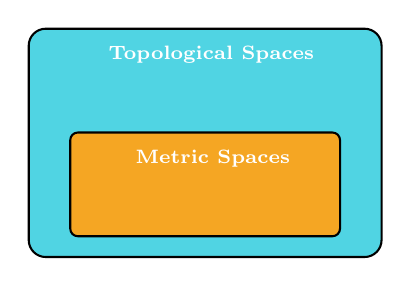
\begin{tikzpicture}[x=0.75pt,y=0.75pt,yscale=-1,xscale=1]
		%uncomment if require: \path (0,300); %set diagram left start at 0, and has height of 300
		
		%Rounded Rect [id:dp8983262620207249] 
		\draw  [fill={rgb, 255:red, 80; green, 212; blue, 227 }  ,fill opacity=1 ] (80,78.2) .. controls (80,73.67) and (83.67,70) .. (88.2,70) -- (241.8,70) .. controls (246.33,70) and (250,73.67) .. (250,78.2) -- (250,171.8) .. controls (250,176.33) and (246.33,180) .. (241.8,180) -- (88.2,180) .. controls (83.67,180) and (80,176.33) .. (80,171.8) -- cycle ;
		%Rounded Rect [id:dp4318601497382968] 
		\draw  [fill={rgb, 255:red, 245; green, 166; blue, 35 }  ,fill opacity=1 ] (100,123.73) .. controls (100,121.67) and (101.67,120) .. (103.73,120) -- (226.27,120) .. controls (228.33,120) and (230,121.67) .. (230,123.73) -- (230,166.27) .. controls (230,168.33) and (228.33,170) .. (226.27,170) -- (103.73,170) .. controls (101.67,170) and (100,168.33) .. (100,166.27) -- cycle ;
		
		% Text Node
		\draw (117,77) node [anchor=north west][inner sep=0.75pt]  [font=\scriptsize] [align=left] {\textcolor[rgb]{1,1,1}{\textbf{Topological Spaces}}};
		% Text Node
		\draw (130,127) node [anchor=north west][inner sep=0.75pt]  [font=\scriptsize,color={rgb, 255:red, 255; green, 255; blue, 255 }  ,opacity=1 ] [align=left] {\textbf{Metric Spaces}};
		
		
	\end{tikzpicture}
\end{center}